\chapter{Centro de compostaje}

La práctica del compostaje consiste en la descomposición controlada de materia orgánica por organismos descomponedores (tales como bacterias, hongos y algunos insectos), y tiene como resultado un producto que puede servir como abono y regenerador de suelos, esto por todos los nutrientes que este aporta al sustrato y a las plantas en él. Este proceso ofrece un método sustentable del manejo de residuos, pues les da una segunda vida útil que apoya el uso de los suelos, ya sea para uso humano o para la conservación de la naturaleza.

El centro de compostaje propuesto estará basado en técnicas de compostaje comunitario y en trabajo voluntario por parte de los alumnos de la universidad. Su manejo de residuos se centrará en residuos creados dentro de la universidad, en locales cercanos y en los hogares de los alumnos, y el uso del abono puede ser tanto para la fertilización de áreas verdes universitarias como para prácticas académicas.

Se espera que este programa ayude a formar de mejor manera a los estudiantes con carreras afines a la práctica del compostaje y fomente estilos de vida más sustentables entre la comunidad universitaria.


\section{Procesamiento de residuos del centro de compostaje}

\subsection{Obtención}

La materia prima necesaria para la realización de la composta será recolectada por 3 medios:

\begin{itemize}
    \item Separación de una parte de los residuos universitarios.
    \item Contenedores en locales cercanos a la universidad.
    \item Un programa de recolección de donaciones de residuos orgánicos recolectados por los alumnos en sus hogares.
\end{itemize}

\subsubsection{Separación de residuos universitarios}


La principal fuente de material compostable serían los residuos de alimentos generados en la cafetería de la universidad, la cual tiene una producción aproximada de residuos compostables de 10 litros semanales.

Otra fuente de material compostable dentro de la universidad son los residuos de papel para manos en baños. Estos residuos llegan a tener una producción aproximada de 4 bolsas diarias, y puesto que no se mezclan con otros residuos, presentan una fácil recolección. Se planea acordar con el personal de limpieza que tales bolsas sean apartadas en su recolección para que posteriormente el voluntario encargado las lleve al centro de compostaje, donde serán almacenadas en bolsas grandes hasta que se necesiten.

Otra fuente de material seco podría ser la vegetación seca producida por las áreas verdes de la universidad. La separación de tales residuos podría realizarse de dos formas:

\begin{enumerate}
    \item Manteniendo comunicación entre el equipo de poda de la universidad y el club de compostaje para que sean estos últimos quienes transporten los residuos.
    \item Realizando actividades de limpieza de áreas verdes apoyadas por alumnos voluntarios.
\end{enumerate}


\subsubsection{Contenedores para recolección de residuos orgánica en comercios cercanos}

La principal fuente de basura orgánica serán una serie de contenedores exclusivos para recolectar basura orgánica, los cuales se colocarán en locales de comida cercano a la universidad.

    \begin{table}[H]

\caption{Ubicaciones para recolectar residuos orgánicos y cantidad aproximada}
\label{tab:ubicaciones_para_contenedores}

\begin{threeparttable}

{\small\setstretch{1.5}\rowcolors{2}{Acento}{White}

\begin{tabular}{M{0.3\linewidth}M{0.3\linewidth}M{0.3\linewidth}}\hline
    
    \theader{Lugar} & \theader{Tipo de basura} & \theader{Cantidad} \\ \hline

    Local - 1  & Frutas y verduras & 5-15 Lt. diarios \\
    Local - 2 & Restos de tomate y cebolla & 0-4 Lt. diarios \\
    Dobby’s Café & Restos de café  & 2 Lt. semanales \\

    \hline
\end{tabular}

}

\begin{tablenotes}\tiny % ex: \tnote{1} ... \item[1]
    \item[1] 
\end{tablenotes}

\end{threeparttable}
\end{table}
    
\subsubsection{Programa de donaciones de residuos de hogares}

Para un mayor involucramiento de los estudiantes y una mejor promoción de la práctica de la separación de residuos, uno de los contenedores construidos será establecido en la entrada de la universidad para que las personas puedan depositar la basura orgánica que separen en sus hogares. Los contenedores contarán con medios a través del cuál las personas podrán registrar sus donaciones (código QR y contactos del encargado). Al finalizar el periodo de composta, se le entregará a las personas donantes ⅓ del peso de sus donaciones en forma de composta lista para ser usada.

A futuro se propone también realizar pequeñas cajas especiales para el almacenaje de basura orgánica, las cuales se venderán a las personas para que puedan recoger los residuos orgánicos de su hogar con mayor facilidad.

\subsection{Procesamiento}

\begin{figure}
    \centering
    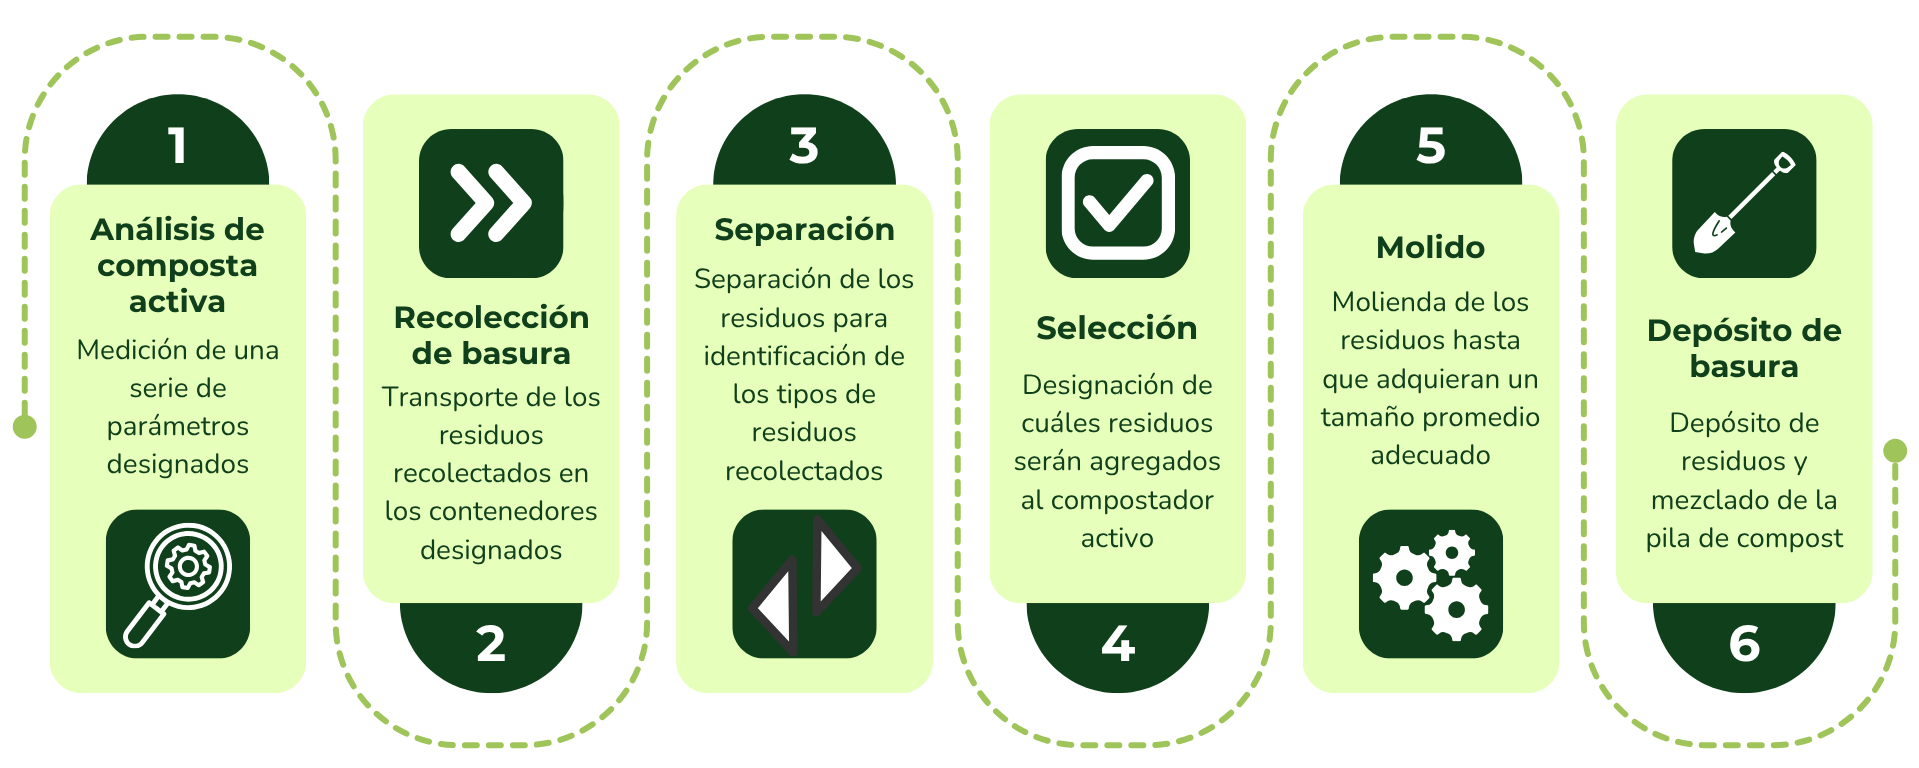
\includegraphics[width=0.9\linewidth]{proceso_de_compostaje}
    \textcolor{Primario}{\rule{\linewidth}{0.5pt}}
    \caption{Proceso de compostaje}
    \label{fig:proceso_de_compostaje}
\end{figure}

El centro de compostaje operará a través de la siguiente serie de pasos (\autoref{fig:proceso_de_compostaje}):

\begin{enumerate}
    \item Análisis: En algún momento previo al depósito de la basura, se tomarán mediciones de los siguientes valores en todos los compostadores y serán subidos a una base de datos designada.
        \subitem Temperatura
        \subitem pH
        \subitem Oxigenación
        \subitem Humedad
        \subitem Compactación
    \item Recolección de basura: El primer paso será transportar de manera diaria la basura orgánica que se haya recolectado en los contenedores especiales. La metodología exacta puede variar entre contenedores debido a sus diferentes características y ubicaciones.
    \item Separación: Una vez recolectada la basura en el centro de compostaje, esta se separará para tener un registro de su composición, elegir de manera más precisa la basura que será depositada en el compostador y desechar la basura que no es compostable.
    \item Determinación de basura a depositar: Se revisará la base de datos del compost en procesamiento para determinar qué basura será agregada al compostador activo. Se tomará entonces la basura seleccionada, y la que no será usada se desechará. La basura que si será agregada será registrada en la base de datos del compostador activo.
    \item Molido: Una vez determinado el conjunto que se agregará, éste se molerá hasta que adquiera un tamaño promedio adecuado.
    \item Depósito de basura: Se depositará en el compostador activo la basura previamente procesada y se añadirá una porción de igual volumen de material estructurante (también molido). Por último, se mezclará la composta hasta que todos los materiales se integren bien.
\end{enumerate}


\subsubsection{Ciclo de operación}

El centro de compostaje operará en base al método más básico de compostaje, el método de volteo. Este método consiste en delimitar un área donde se depositarán de manera constante los residuos orgánicos, para posteriormente realizar un volteo. La adición de residuos se realizará durante 1 mes. Una vez alcanzado el mes, se mezclará bien la pila de composta y se dejará en un proceso de maduración durante 3 meses.

Pasados los 3 meses de maduración de un lote, éste será retirado de su contenedor para pasar por un tamizado y posteriormente se le dará uso.

Aquel contenido que no tenga un uso inmediato será conservado en costales en un área designada.

\subsection{Usos}

\subsubsection{Programa de donaciones de residuos de hogares}

Como se mencionó anteriormente, existirá un contenedor en el cual los alumnos podrán donar residuos que decidan separar en sus hogares. Estas donaciones serán pesadas y registradas en el lugar del contenedor.

La última semana de la etapa de maduración de un lote se consultarán los datos del registro de donaciones de tal lote para identificar a los alumnos, determinar la cantidad de composta que recibirá cada uno ($\frac{1}{2}$ del peso total de sus donaciones) y convocarlos a la fecha y lugar designados en que se realizará la entrega de composta.

\subsubsection{Prácticas académicas}

Como producto biológico que es el compost, estudiantes y docentes de la universidad pueden encontrar en el centro de compostaje un espacio en el cual pueden realizar prácticas para un mejor aprendizaje en sus materias, así como hacer uso del compost resultante para prácticas relacionadas a la mejora de suelos.

Las licenciaturas más beneficiadas podrían ser: Biotecnología, Energía y desarrollo sostenible y Tecnología ambiental y sustentabilidad.

\subsubsection{Áreas verdes universitarias}

El compostaje producido puede ser también utilizado por la universidad para la fertilización de sus áreas verdes.

\section{Infraestructura del centro de compostaje}

\subsection{Contenedores para negocios}

Los contenedores serán construidos de madera de tarimas reciclada, sin embargo, en su interior estos contarán con un recubrimiento de láminas de pvc recicladas para que no existan escurrimientos o salidas de malos olores. De igual manera, algunos contenedores tendrán cinta magnética en el contorno de su tapa para que cierren sin dejar salir olores. Otras consideración a tomar en cuenta será colocarles etiquetas con información sobre materiales a compostar, así como ruedas para una mejor movilidad.

La construcción exacta de los contenedores dependerá del lugar en que se coloquen.

\subsubsection{Contenedor de donaciones}

Se planea colocar también un contenedor dedicado a recibir las donaciones de los alumnos que decidan separar los residuos orgánicos compostables de sus hogares.

Será construido, de igual manera, a base de madera reciclada, con un recubrimiento interior de láminas de PVC para evitar el impacto de la humedad de los residuos y con una tapa para evitar la salida de malos olores,

Contará también con una báscula para que los alumnos puedan registrar el peso de sus donaciones. Este registro será realizado por medio de un código QR que los dirija a una  encuesta en Google Forms en la que se les pedirá, además del peso de su donación, algún dato de identificación como lo puede ser su nombre, carrera y grupo, o directamente su matrícula.

\subsection{Equipos y materiales}

El mantenimiento del centro de compostaje dependerá no solo del trabajo de los voluntarios, sino también de que estos cuenten con los equipos  y herramientas necesarios para realizar las actividades.

    % \input{Lista de equipos y herramientas}
    
\subsection{Ubicaciones propuestas para el centro de compostaje}

    % PENDIENTE
    
